%\input{Preambulum}

\begin{figure}[t!]
\centering
\begin{subfigure}{0.24\textwidth}
\centering
\caption{$I_1$: \#12714}
\label{Fig7a}

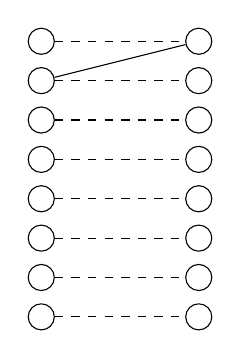
\begin{tikzpicture}[scale=1, auto=center]
\tikzstyle{every node}=[draw,shape=circle];
  \node[minimum size=0.25cm] (n1) at (0,3.5) {};
  \node[minimum size=0.25cm] (n2) at (0,3)   {};
  \node[minimum size=0.25cm] (n3) at (0,2.5) {};
  \node[minimum size=0.25cm] (n4) at (0,2)   {};
  \node[minimum size=0.25cm] (n5) at (0,1.5) {};
  \node[minimum size=0.25cm] (n6) at (0,1)   {};
  \node[minimum size=0.25cm] (n7) at (0,0.5) {};
  \node[minimum size=0.25cm] (n8) at (0,0)   {};
  \node[minimum size=0.25cm] (n9) at (2,3.5) {};
  \node[minimum size=0.25cm] (n10) at (2,3)   {};
  \node[minimum size=0.25cm] (n11) at (2,2.5) {};
  \node[minimum size=0.25cm] (n12) at (2,2)   {};
  \node[minimum size=0.25cm] (n13) at (2,1.5) {};
  \node[minimum size=0.25cm] (n14) at (2,1)   {};
  \node[minimum size=0.25cm] (n15) at (2,0.5) {};
  \node[minimum size=0.25cm] (n16) at (2,0)   {};

  \foreach \from/\to in {n1/n9,n2/n10,n3/n11,n4/n12,n5/n13,n6/n14,n7/n15,n8/n16}
    \draw[dashed] (\from) -- (\to);
  \foreach \from/\to in {n2/n9}
    \draw (\from) -- (\to);
\end{tikzpicture}
\end{subfigure}
\begin{subfigure}{0.24\textwidth}
\centering
\caption{$I_2$: \#10904}
\label{Fig7b}

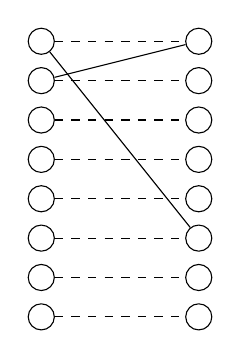
\begin{tikzpicture}[scale=1, auto=center]
\tikzstyle{every node}=[draw,shape=circle];
  \node[minimum size=0.25cm] (n1) at (0,3.5) {};
  \node[minimum size=0.25cm] (n2) at (0,3)   {};
  \node[minimum size=0.25cm] (n3) at (0,2.5) {};
  \node[minimum size=0.25cm] (n4) at (0,2)   {};
  \node[minimum size=0.25cm] (n5) at (0,1.5) {};
  \node[minimum size=0.25cm] (n6) at (0,1)   {};
  \node[minimum size=0.25cm] (n7) at (0,0.5) {};
  \node[minimum size=0.25cm] (n8) at (0,0)   {};
  \node[minimum size=0.25cm] (n9) at (2,3.5) {};
  \node[minimum size=0.25cm] (n10) at (2,3)   {};
  \node[minimum size=0.25cm] (n11) at (2,2.5) {};
  \node[minimum size=0.25cm] (n12) at (2,2)   {};
  \node[minimum size=0.25cm] (n13) at (2,1.5) {};
  \node[minimum size=0.25cm] (n14) at (2,1)   {};
  \node[minimum size=0.25cm] (n15) at (2,0.5) {};
  \node[minimum size=0.25cm] (n16) at (2,0)   {};

  \foreach \from/\to in {n1/n9,n2/n10,n3/n11,n4/n12,n5/n13,n6/n14,n7/n15,n8/n16}
    \draw[dashed] (\from) -- (\to);
  \foreach \from/\to in {n1/n14,n2/n9}
    \draw (\from) -- (\to);
\end{tikzpicture}
\end{subfigure}
\begin{subfigure}{0.24\textwidth}
\centering
\caption{$I_3$: \#9094}
\label{Fig7c}

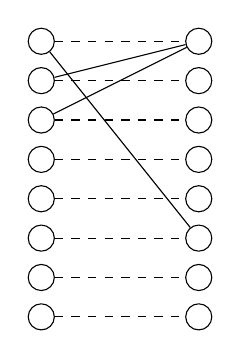
\begin{tikzpicture}[scale=1, auto=center]
\tikzstyle{every node}=[draw,shape=circle];
  \node[minimum size=0.25cm] (n1) at (0,3.5) {};
  \node[minimum size=0.25cm] (n2) at (0,3)   {};
  \node[minimum size=0.25cm] (n3) at (0,2.5) {};
  \node[minimum size=0.25cm] (n4) at (0,2)   {};
  \node[minimum size=0.25cm] (n5) at (0,1.5) {};
  \node[minimum size=0.25cm] (n6) at (0,1)   {};
  \node[minimum size=0.25cm] (n7) at (0,0.5) {};
  \node[minimum size=0.25cm] (n8) at (0,0)   {};
  \node[minimum size=0.25cm] (n9) at (2,3.5) {};
  \node[minimum size=0.25cm] (n10) at (2,3)   {};
  \node[minimum size=0.25cm] (n11) at (2,2.5) {};
  \node[minimum size=0.25cm] (n12) at (2,2)   {};
  \node[minimum size=0.25cm] (n13) at (2,1.5) {};
  \node[minimum size=0.25cm] (n14) at (2,1)   {};
  \node[minimum size=0.25cm] (n15) at (2,0.5) {};
  \node[minimum size=0.25cm] (n16) at (2,0)   {};

  \foreach \from/\to in {n1/n9,n2/n10,n3/n11,n4/n12,n5/n13,n6/n14,n7/n15,n8/n16}
    \draw[dashed] (\from) -- (\to);
  \foreach \from/\to in {n1/n14,n2/n9,n3/n9}
    \draw (\from) -- (\to);
\end{tikzpicture}
\end{subfigure}
\begin{subfigure}{0.24\textwidth}
\centering
\caption{$I_4$: \#7858}
\label{Fig7d}

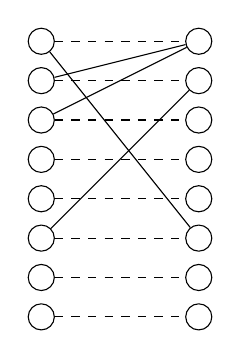
\begin{tikzpicture}[scale=1, auto=center]
\tikzstyle{every node}=[draw,shape=circle];
  \node[minimum size=0.25cm] (n1) at (0,3.5) {};
  \node[minimum size=0.25cm] (n2) at (0,3)   {};
  \node[minimum size=0.25cm] (n3) at (0,2.5) {};
  \node[minimum size=0.25cm] (n4) at (0,2)   {};
  \node[minimum size=0.25cm] (n5) at (0,1.5) {};
  \node[minimum size=0.25cm] (n6) at (0,1)   {};
  \node[minimum size=0.25cm] (n7) at (0,0.5) {};
  \node[minimum size=0.25cm] (n8) at (0,0)   {};
  \node[minimum size=0.25cm] (n9) at (2,3.5) {};
  \node[minimum size=0.25cm] (n10) at (2,3)   {};
  \node[minimum size=0.25cm] (n11) at (2,2.5) {};
  \node[minimum size=0.25cm] (n12) at (2,2)   {};
  \node[minimum size=0.25cm] (n13) at (2,1.5) {};
  \node[minimum size=0.25cm] (n14) at (2,1)   {};
  \node[minimum size=0.25cm] (n15) at (2,0.5) {};
  \node[minimum size=0.25cm] (n16) at (2,0)   {};

  \foreach \from/\to in {n1/n9,n2/n10,n3/n11,n4/n12,n5/n13,n6/n14,n7/n15,n8/n16}
    \draw[dashed] (\from) -- (\to);
  \foreach \from/\to in {n1/n14,n2/n9,n3/n9,n6/n10}
    \draw (\from) -- (\to);
\end{tikzpicture}
\end{subfigure}

\vspace{0.25cm}
\begin{subfigure}{0.24\textwidth}
\centering
\caption{$I_5$: \#6357}
\label{Fig7e}

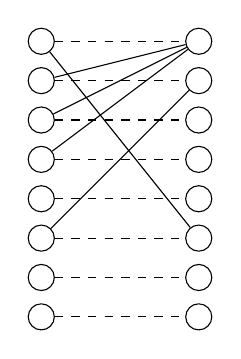
\begin{tikzpicture}[scale=1, auto=center]
\tikzstyle{every node}=[draw,shape=circle];
  \node[minimum size=0.25cm] (n1) at (0,3.5) {};
  \node[minimum size=0.25cm] (n2) at (0,3)   {};
  \node[minimum size=0.25cm] (n3) at (0,2.5) {};
  \node[minimum size=0.25cm] (n4) at (0,2)   {};
  \node[minimum size=0.25cm] (n5) at (0,1.5) {};
  \node[minimum size=0.25cm] (n6) at (0,1)   {};
  \node[minimum size=0.25cm] (n7) at (0,0.5) {};
  \node[minimum size=0.25cm] (n8) at (0,0)   {};
  \node[minimum size=0.25cm] (n9) at (2,3.5) {};
  \node[minimum size=0.25cm] (n10) at (2,3)   {};
  \node[minimum size=0.25cm] (n11) at (2,2.5) {};
  \node[minimum size=0.25cm] (n12) at (2,2)   {};
  \node[minimum size=0.25cm] (n13) at (2,1.5) {};
  \node[minimum size=0.25cm] (n14) at (2,1)   {};
  \node[minimum size=0.25cm] (n15) at (2,0.5) {};
  \node[minimum size=0.25cm] (n16) at (2,0)   {};

  \foreach \from/\to in {n1/n9,n2/n10,n3/n11,n4/n12,n5/n13,n6/n14,n7/n15,n8/n16}
    \draw[dashed] (\from) -- (\to);
  \foreach \from/\to in {n1/n14,n2/n9,n3/n9,n4/n9,n6/n10}
    \draw (\from) -- (\to);
\end{tikzpicture}
\end{subfigure}
\begin{subfigure}{0.24\textwidth}
\centering
\caption{$I_6$: \#5430}
\label{Fig7f}

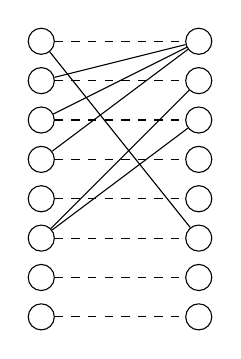
\begin{tikzpicture}[scale=1, auto=center]
\tikzstyle{every node}=[draw,shape=circle];
  \node[minimum size=0.25cm] (n1) at (0,3.5) {};
  \node[minimum size=0.25cm] (n2) at (0,3)   {};
  \node[minimum size=0.25cm] (n3) at (0,2.5) {};
  \node[minimum size=0.25cm] (n4) at (0,2)   {};
  \node[minimum size=0.25cm] (n5) at (0,1.5) {};
  \node[minimum size=0.25cm] (n6) at (0,1)   {};
  \node[minimum size=0.25cm] (n7) at (0,0.5) {};
  \node[minimum size=0.25cm] (n8) at (0,0)   {};
  \node[minimum size=0.25cm] (n9) at (2,3.5) {};
  \node[minimum size=0.25cm] (n10) at (2,3)   {};
  \node[minimum size=0.25cm] (n11) at (2,2.5) {};
  \node[minimum size=0.25cm] (n12) at (2,2)   {};
  \node[minimum size=0.25cm] (n13) at (2,1.5) {};
  \node[minimum size=0.25cm] (n14) at (2,1)   {};
  \node[minimum size=0.25cm] (n15) at (2,0.5) {};
  \node[minimum size=0.25cm] (n16) at (2,0)   {};

  \foreach \from/\to in {n1/n9,n2/n10,n3/n11,n4/n12,n5/n13,n6/n14,n7/n15,n8/n16}
    \draw[dashed] (\from) -- (\to);
  \foreach \from/\to in {n1/n14,n2/n9,n3/n9,n4/n9,n6/n10,n6/n11}
    \draw (\from) -- (\to);
\end{tikzpicture}
\end{subfigure}
\begin{subfigure}{0.24\textwidth}
\centering
\caption{$I_7$: \#4238}
\label{Fig7g}

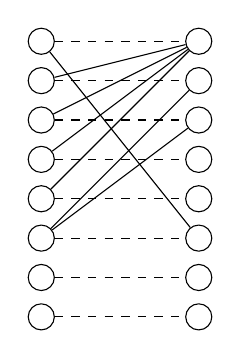
\begin{tikzpicture}[scale=1, auto=center]
\tikzstyle{every node}=[draw,shape=circle];
  \node[minimum size=0.25cm] (n1) at (0,3.5) {};
  \node[minimum size=0.25cm] (n2) at (0,3)   {};
  \node[minimum size=0.25cm] (n3) at (0,2.5) {};
  \node[minimum size=0.25cm] (n4) at (0,2)   {};
  \node[minimum size=0.25cm] (n5) at (0,1.5) {};
  \node[minimum size=0.25cm] (n6) at (0,1)   {};
  \node[minimum size=0.25cm] (n7) at (0,0.5) {};
  \node[minimum size=0.25cm] (n8) at (0,0)   {};
  \node[minimum size=0.25cm] (n9) at (2,3.5) {};
  \node[minimum size=0.25cm] (n10) at (2,3)   {};
  \node[minimum size=0.25cm] (n11) at (2,2.5) {};
  \node[minimum size=0.25cm] (n12) at (2,2)   {};
  \node[minimum size=0.25cm] (n13) at (2,1.5) {};
  \node[minimum size=0.25cm] (n14) at (2,1)   {};
  \node[minimum size=0.25cm] (n15) at (2,0.5) {};
  \node[minimum size=0.25cm] (n16) at (2,0)   {};

  \foreach \from/\to in {n1/n9,n2/n10,n3/n11,n4/n12,n5/n13,n6/n14,n7/n15,n8/n16}
    \draw[dashed] (\from) -- (\to);
  \foreach \from/\to in {n1/n14,n2/n9,n3/n9,n4/n9,n5/n9,n6/n10,n6/n11}
    \draw (\from) -- (\to);
\end{tikzpicture}
\end{subfigure}
\begin{subfigure}{0.24\textwidth}
\centering
\caption{$I_8$: \#3759}
\label{Fig7h}

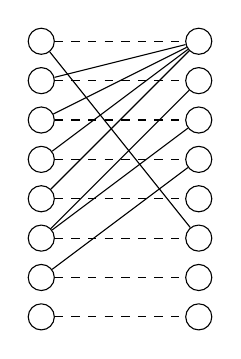
\begin{tikzpicture}[scale=1, auto=center]
\tikzstyle{every node}=[draw,shape=circle];
  \node[minimum size=0.25cm] (n1) at (0,3.5) {};
  \node[minimum size=0.25cm] (n2) at (0,3)   {};
  \node[minimum size=0.25cm] (n3) at (0,2.5) {};
  \node[minimum size=0.25cm] (n4) at (0,2)   {};
  \node[minimum size=0.25cm] (n5) at (0,1.5) {};
  \node[minimum size=0.25cm] (n6) at (0,1)   {};
  \node[minimum size=0.25cm] (n7) at (0,0.5) {};
  \node[minimum size=0.25cm] (n8) at (0,0)   {};
  \node[minimum size=0.25cm] (n9) at (2,3.5) {};
  \node[minimum size=0.25cm] (n10) at (2,3)   {};
  \node[minimum size=0.25cm] (n11) at (2,2.5) {};
  \node[minimum size=0.25cm] (n12) at (2,2)   {};
  \node[minimum size=0.25cm] (n13) at (2,1.5) {};
  \node[minimum size=0.25cm] (n14) at (2,1)   {};
  \node[minimum size=0.25cm] (n15) at (2,0.5) {};
  \node[minimum size=0.25cm] (n16) at (2,0)   {};

  \foreach \from/\to in {n1/n9,n2/n10,n3/n11,n4/n12,n5/n13,n6/n14,n7/n15,n8/n16}
    \draw[dashed] (\from) -- (\to);
  \foreach \from/\to in {n1/n14,n2/n9,n3/n9,n4/n9,n5/n9,n6/n10,n6/n11,n7/n12}
    \draw (\from) -- (\to);
\end{tikzpicture}
\end{subfigure}

\caption{Some balanced bipartite graphs with \\
16 nodes and an increasing set of exclusions \\ \vspace{0.2cm}
\footnotesize{\emph{Notes}: Dashed lines indicate the group constraints, solid lines indicate the association constraints. \\
Group winners are the nodes on the left-hand side, runners-up are the nodes on the right-hand side. \\
\# = number of valid assignments}}
\label{Fig7}
\end{figure}

%\end{document}